\chapter{Theoretische Achtergrond}
\label{hst-theorie}
Om de gebruikte aanpak zo goed mogelijk te begrijpen zijn een aantal theoretische concepten nodig. Dit hoofdstuk biedt een overzicht van de belangrijkste gebruikte methodes en technieken in dit onderzoek.

Een eerste sectie bespreekt de neurale netwerken die afbeeldingen voorstellen en zinnen kunnen genereren. De tweede sectie focust op twee statistische concepten die zijn aangewend om extra semantische informatie uit afbeeldingen te extraheren. 

\section{Neurale Netwerken}
Algemeen dient een neuraal netwerk als een simulatie van menselijke hersenen. De structuur van een neuraal netwerk bootst de werking van de neuronen en synapsen in het menselijke brein na. 

Neuronen zijn de primitieve eenheden van het menselijke zenuwstelsel. Ze staan in verbinding met elkaar door middel van synapsen en communiceren met behulp van elektrische potentiaal. Afhankelijk van de aan- of afwezigheid van potentiaal over de inkomende verbindingen stuurt een neuron al dan niet een signaal door naar het volgende neuron. Deze eenheden zijn zeer makkelijk softwarematig te simuleren.

Elk artificieel neuraal netwerk heeft een trainingsfase nodig waarin het de juiste gewichten voor alle verbindingen leert. Deze gewichten simuleren de gevoeligheid voor potentiaal van een inkomende verbinding. Na de training kan het netwerk ongeziene input omvormen tot de juiste output.

Deze sectie geeft een inleiding tot de gebruikte neurale netwerken. Een eerste deel handelt over het eenvoudigste type neuraal netwerk (feedforward), dat de basis vormt voor een aantal gebruikte varianten. Daarna volgt een toelichting van enkele meer complexe netwerken: recurrente en convolutionele neurale netwerken, alsook Long Short Term Memory netwerken.

\subsection{Feedforward Neurale Netwerken}
\subsubsection{Perceptron} % (fold)
\label{par:perceptron}

Om een feedforward neuraal netwerk te begrijpen is het concept perceptron nodig. Dit is een netwerk bestaande uit \'e\'en of meer neuronen, met \'e\'en of meerdere inputs ($x_i$). De output $y$ van een neuron is een gewogen som van alle inputs met gewichten $w_i$, al dan niet gewijzigd door een transferfunctie $f$ (formule \ref{formule:neuron}). Typische voorbeelden van transferfuncties zijn de logistische functie en de hyperbolische tangensfunctie.

\begin{equation}
    y = f(\sum\limits_{i=1}^{n}w_i x_i)
    \label{formule:neuron}
\end{equation}

Het is ook mogelijk om een perceptron met meerdere outputs te gebruiken. Hierbij hebben alle verbindingen tussen in- en outputs een eigen gewicht en kan elke output een verschillende transferfunctie hebben. Figuur \ref{fig:perceptron} toont een perceptron met vijf inputs en drie outputs. Deze architectuur komt exact overeen met drie aparte neuronen die allemaal dezelfde inputs krijgen, maar elk verschillende gewichten en een verschillende transferfunctie $f_i$ gebruiken.

\begin{figure}[ht]
\def\layersep{2.5cm}
\centering
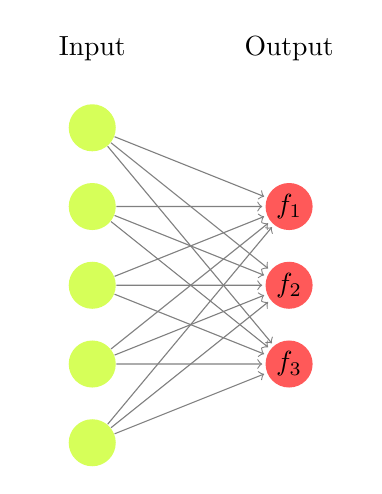
\begin{tikzpicture}[shorten >=1pt,->,draw=black!50, node distance=\layersep]
    \tikzstyle{every pin edge}=[<-,shorten <=1pt]
    \tikzstyle{neuron}=[circle,fill=black!100,minimum size=17pt,inner sep=0pt]
    \tikzstyle{input neuron}=[neuron, fill=lime!65];
    \tikzstyle{output neuron}=[neuron, fill=red!65];
    \tikzstyle{annot} = [text width=4em, text centered]

    %input neurons
    \foreach \name / \y in {1,...,5}
        \path[yshift=0.5cm]
            node[input neuron] (I-\name) at (0,-\y cm){};

    %output neurons
    \foreach \name / \y in {1,...,3}
        \node[output neuron] (O-\name) at (\layersep,-\y-0.5) {$f_{\name}$};

    %links
    \foreach \source in {1,...,5}
        \foreach \dest in {1,...,3}
            \path (I-\source) edge (O-\dest);

    % Annotate the layers
    \node[annot,above of=I-1, node distance=1cm] (i1) {Input};
    \node[annot,right of=i1] (hl2) {Output};
\end{tikzpicture}
\caption{Perceptron met vijf inputs en drie outputs}
\label{fig:perceptron}
\end{figure}


\subsubsection{Feedforward Netwerk}
\label{par:concept}
Een feedforward neuraal netwerk is \'e\'en van de eenvoudigste neurale netwerken. Het is een perceptron met \'e\'en of meer verborgen lagen van neuronen tussen input en output. De outputs van elke laag worden enkel doorgegeven aan de volgende laag, er zijn dus geen cycli in het netwerk (zie figuur \ref{fig:ffnn}). Elke pijl op de figuur vertegenwoordigt een vermenigvuldiging met een bepaald gewicht. Dit gewicht is een natuurlijk getal. Het is ook mogelijk om gewichten te hebben met waarden nul, waardoor de volgende laag niet volledig verbonden is. Het is voor elke knoop in het netwerk bovendien mogelijk om een transferfunctie te gebruiken alvorens de waarde door te sturen naar de volgende laag. Het netwerk kan ook een outputlaag te gebruiken met meerdere knopen, wat neerkomt op een parallelle uitvoering van meerdere netwerken met een enkele output\cite{Bishop:1995:NNP:525960}.

\begin{figure}[ht]
\def\layersep{2.5cm}
\centering
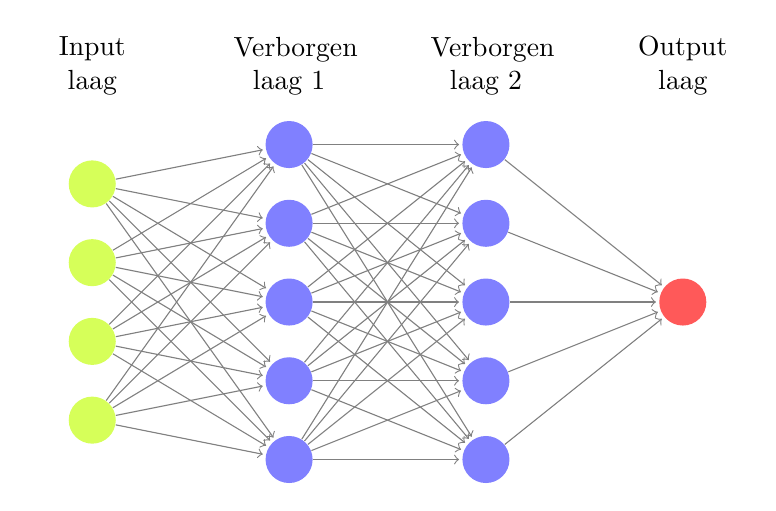
\begin{tikzpicture}[shorten >=1pt,->,draw=black!50, node distance=\layersep]
    \tikzstyle{every pin edge}=[<-,shorten <=1pt]
    \tikzstyle{neuron}=[circle,fill=black!25,minimum size=17pt,inner sep=0pt]
    \tikzstyle{input neuron}=[neuron, fill=lime!65];
    \tikzstyle{output neuron}=[neuron, fill=red!65];
    \tikzstyle{verborgen neuron}=[neuron, fill=blue!50];
    \tikzstyle{annot} = [text width=4em, text centered]

    % Draw the input layer nodes
    \foreach \name / \y in {1,...,4}
    % This is the same as writing \foreach \name / \y in {1/1,2/2,3/3,4/4}
        \node[input neuron] (I-\name) at (0,-\y) {};

    % Draw the hidden layer nodes
    \foreach \name / \y in {1,...,5}
        \path[yshift=0.5cm]
            node[verborgen neuron] (H1-\name) at (\layersep,-\y cm) {};

    % Draw the hidden layer nodes
    \foreach \name / \y in {1,...,5}
        \path[yshift=0.5cm]
            node[verborgen neuron] (H2-\name) at (2*\layersep,-\y cm) {};

    % Draw the output layer node
    \node[output neuron, right of=H2-3] (O) {};

    % Connect every node in the input layer with every node in the
    % hidden layer.
    \foreach \source in {1,...,4}
        \foreach \dest in {1,...,5}
            \path (I-\source) edge (H1-\dest);
    %links van eerste naar tweede hidden layer
    \foreach \source in {1,...,5}
        \foreach \dest in {1,...,5}
            \path (H1-\source) edge (H2-\dest);

    % Connect every node in the hidden layer with the output layer
    \foreach \source in {1,...,5}
        \path (H2-\source) edge (O);

    % Annotate the layers
    \node[annot,above of=H1-1, node distance=1cm] (hl1) {Verborgen laag 1};
    \node[annot,above of=H2-1, node distance=1cm] (hl2) {Verborgen laag 2};
    \node[annot,left of=hl1] {Input laag};
    \node[annot,right of=hl2] {Output laag};
\end{tikzpicture}
\caption{Feedforward neuraal netwerk met twee verborgen lagen}
\label{fig:ffnn}
\end{figure}

% subsubsection concept (end)

\subsubsection{Training} % (fold)
\label{par:training}
Het trainen van een feedforward netwerk gebeurt meestal met terugpropagatie. Deze techniek vergelijkt voor elke input de berekende met de verwachte outputwaarde. Op basis van dit verschil gebeuren er aanpassingen aan de gewichten van het netwerk. Deze aanpassingen propageren in omgekeerde volgorde doorheen het netwerk: ze beginnen bij de gewichten van de laatste laag, daarna de voorlaatste,\ldots 

Voor een netwerk met \'e\'en verborgen laag geldt het volgende voor de waarden van de verborgen knopen $\mathbf{\hat{h}}$ en voorspelde outputvector $\mathbf{\hat{y}}$ bij inputvector $\mathbf{x}$:
\begin{equation}
    \mathbf{\hat{h}} = f(\mathbf{Wx})
\end{equation}
\begin{equation}
    \boldsymbol{\hat{y}} = f(\boldsymbol{W'\hat{h}}) = f(\boldsymbol{\hat{h}'}) = f(\boldsymbol{W'}f(\boldsymbol{Wx}))
\end{equation}
waarbij $\mathbf{W}$ en $\mathbf{W'}$ de gewichten van de verbindingen tussen respectievelijk de input en de verborgen laag, en de verborgen laag en de output voorstellen. $f$ is telkens de transferfunctie. In deze formule is ze gelijk voor elke laag, maar het is mogelijk om voor elke laag een andere functie te gebruiken.

Het probleem bij het leren van $\mathbf{W}$ en $\mathbf{W'}$ is dat de correcte verborgen vector $\mathbf{h}$ niet gekend is. De training van het netwerk kan dus enkel op basis van de input, de  berekende output en de verwachte output gebeuren.

Een eerste stap is het verkleinen van het verschil $\mathbf{\hat{y}} - \mathbf{y}$ door het aanpassen van \myvector{W'} en \myvector{\hat{h}}. \myvector{W'} wordt gewijzigd met behulp van gradient descent, veronderstellende dat \myvector{\hat{h}} correct is. Gradient descent is een eenvoudig optimalisatie algoritme dat kan dienen om het lokale minimum van een functie te vinden. De minimalisatie gebeurt op een ``gulzige'' manier, door elke stap wijzigingen aan te brengen in de richting van de steilste afdaling. Deze richting komt overeen met de eerste afgeleide van de transferfunctie, berekend in alle variabelen van de output van het netwerk:

\begin{equation}
df_i = \frac{\partial}{\partial\hat{h_i}'}f(\hat{h_i}')
\end{equation}
In het geval van een logistische transferfunctie $f(x) = \frac{1}{1 + \mathrm e^{-x}}$ geeft dit volgende vector van afgeleiden:
\begin{equation}
  \mathbf{df} = \frac{d}{d\hat{h}'}\mathbf{\hat{y}} = \mathbf{\hat{y}}(1-\mathbf{\hat{y}})
\end{equation}

De formule om de gewichten te updaten ziet er in het algemene geval uit als volgt:
\begin{equation}
  w'_{ji} = w'_{ji} + \sigma(y_j-\hat{y}_j)df_i\hat{h}_i
\end{equation}
Hierbij stelt $\sigma$ de leersnelheid (learning rate) voor. De leersnelheid bepaalt hoe zwaar de aanpassing aan de gewichten doorweegt.
Indien het netwerkt met een logistische transferfunctie werkt, geeft dit het volgende resultaat:
\begin{equation}
    w'_{ji} = w'_{ji} + \sigma(y_j-\hat{y}_j)\hat{y}_j(1-\hat{y}_j)\hat{h}_i
\end{equation}
Bij elke stap zorgt de gradi\"ent ervoor dat na aanpassing van de gewichten, bij dezelfde input, de output dichter bij het gewenste resultaat zal liggen.

Vervolgens zorgt gradient descent voor een aanpassing van \myvector{\hat{h}}. Er kunnen echter geen wijzigingen worden aangebracht in \myvector{\hat{h}} zelf, dus wijzigt het algoritme \myvector{W} op de manier die de fout op \myvector{\hat{h}} het meeste verkleint. Gradient descent leidt tot volgende \myvector{\Delta h}, die de gewenste verandering van \myvector{\hat{h}} weergeeft:
\begin{equation}
    \Delta h_i = \sum\limits_{j}(y_j-\hat{y}_j)\hat{y}_j(1-\hat{y}_j)w'_{ji}
\end{equation}
Op basis van \myvector{\Delta h} en \myvector{\hat{h}} wijzigt het algoritme \myvector{W} met volgende formule:
\begin{equation}
    w_{ji} = w_{ji} + \sigma(\Delta h_j)\hat{h}_j(1-\hat{h}_j)x_i
\end{equation}
Op deze manier verkleint de fout op de output \myvector{\hat{y}-y}, deels door de verandering in \myvector{W} en deels door die in \myvector{W'}\cite{Blockeel}.

Herhaalde toepassing van deze techniek voor elk paar van gekende inputs en outputs zorgt dat het netwerk op termijn de juiste gewichten leert. Het is ook mogelijk om elke input meerdere keren te gebruiken om zo tot een beter resultaat te komen. Om complexere relaties tussen in en output te leren is deze methode zeer eenvoudig uit te breiden naar netwerken met een arbitrair aantal verborgen lagen. Hierbij propageert de fout van elke laag door naar de gewichten van de vorige laag, door gebruik te maken van dezelfde concepten als hierboven beschreven. Terugpropagatie maakt het ook mogelijk om netwerken met complexere structuren te leren, zoals netwerken met terugkoppelingen (RNN) of convolutionele lagen (CNN).
% subsubsection training (end)

\subsubsection{Softmaxlaag}\label{par:softmax}
De softmaxlaag is een laag die vaak als laatste laag in een neuraal netwerk voorkomt. Wanneer het netwerk meerdere outputs heeft, geeft de softmaxlaag een kansverdeling over de verschillende outputs terug in plaats van de oorspronkelijke outputvector. Concreet betekent dit dat het de outputwaarden normaliseert zodat elke waarde positief is en bovendien de som van alle waarden gelijk is aan 1. Dit is bijvoorbeeld nuttig bij het leren van een kansverdeling over een aantal discrete componenten. Ook bij classificatie van input die tegelijkertijd tot meerdere klassen kan behoren is dit van nut.

De berekening van de kansverdeling gebeurt met de softmaxfunctie $s$ in formule \eqref{formula-softmax}. Hierbij is $\mathbf{o}$ de outputvector van grootte $n$.
\begin{equation}
s(\textbf{o})_i = \frac{e^{o_i}}{\sum^{n}_{k=1}{e^{o_k}}}
\label{formula-softmax}
\end{equation}

Het gebruik van de softmaxfunctie bij training met backpropagatie is zeer eenvoudig aangezien de afgeleide zeer simpel te berekenen is. De afgeleide van de softmaxfunctie is te zien in formule \eqref{softmax_derivative}. Hierbij is $\delta_{ik}$ de Kroneckerdelta, die gelijk is aan $1$ als $i = k$ en anders gelijk is aan $0$.

\begin{equation}
    \frac{\partial}{\partial o_k}s(\textbf{o})_i =  s(\textbf{o})_i(\delta_{ik} - s(\textbf{o})_k)
    \label{softmax_derivative}
\end{equation}

Bij het gebruik van negatieve logwaarschijnlijkheid als foutenfunctie ($L$) komt dit neer op volgende zeer eenvoudige afgeleide van de foutenfunctie:

\begin{equation}
    \frac{\partial L}{\partial o_i} = \sum_{k=1}^n{y_i}s(\textbf{o})_i - y_i
\end{equation}
met $\textbf{y}$ de correcte output. Als de outputvector een one-hot codering heeft valt de som in deze formule weg en is de afgeleide in elke component gelijk aan het verschil van de voorspelde en de correcte output\cite{Bishop:1995:NNP:525960}. 

In deze thesis komt een softmax voor als laatste laag bij de gebruikte CNN (sectie \ref{sec:usedcnn}), als laatste laag in het netwerk bij de voorspelling van LDA-topicverdelingen (sectie \ref{sec:LDAprediction}) en als laatste laag in de gebruikte taalnetwerken (sectie \ref{sec:rnn_methodology} en \ref{sec:lstm}).

% CNN
\subsection{Convolutionele Neurale Netwerken}
\label{sec:CNN}
\subsubsection{Concept}
Convolutionele Neurale Netwerken (ConvNets of CNN's) zijn biologisch ge\" inspireerde trainbare architecturen die invariante afbeeldingskarakteristieken kunnen leren\cite{LeCun2010}. Ze bieden een hi\"erarchische representatie van een afbeelding en zijn van nut in tal van visuele taken\cite{Ciresan2012,Girshick2014,Zhou2015}.

Een CNN is een \emph{deep learning} architectuur bestaande uit verschillende niveaus. De input en output van elk niveau is een verzameling van arrays die men een \emph{feature map} noemt. Op elke output is de feature map een representatie van een bepaald kenmerk van de afbeelding. Elk niveau bestaat standaard uit drie lagen: een filter bank laag, een niet-lineaire laag en een feature pooling laag. Na een aantal van deze niveaus is er nog een classificatielaag.

Eerst is er een filter bank laag die een aantal features kan detecteren in de input. In deze filterlaag gebeurt de eigenlijke convolutie. Het netwerk berekent de convolutie van de input \emph{feature map} met een aantal kernelfuncties. Elke filterlaag detecteert andere features op alle mogelijke locaties van de input. Figuur \ref{fig:cnnfilters} toont een voorbeeld van geleerde kernelfuncties na afloop van het trainingsproces. De bovenste drie rijen filters focussen minder op kleur, terwijl de onderste drie rijen dat wel doen.

\begin{figure}[tb]
    \centering
    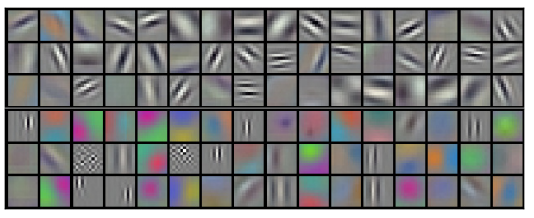
\includegraphics[width=.7\textwidth]{Images/cnnfilters.png}
    \caption{96 convolutionele filters\cite{Krizhevsky2012a}}
    \label{fig:cnnfilters}
\end{figure}

Na de filters volgt een niet-lineaire laag. Deze kan een eenvoudige functie bevatten zoals een sigmo\"ide of de $\tanh$ functie, maar kan ook veel complexer zijn en bijvoorbeeld een ``rectified sigmoid'' bevatten, al dan niet gecombineerd met een normalisatie.

De laatste laag in elk niveau is een feature pooling laag die de dimensionaliteit van de output reduceert door regio's van de output te vervangen door hun gemiddelde of maximumwaarde. De maxima (of gemiddelde waarden) van alle regio's verlagen de dimensie van de input. Figuur \ref{fig:maxpool} illustreert het principe van max-pooling met een filtergrootte van 2x2 en een stapgrootte van 2. 

\begin{figure}[tb]
    \centering
    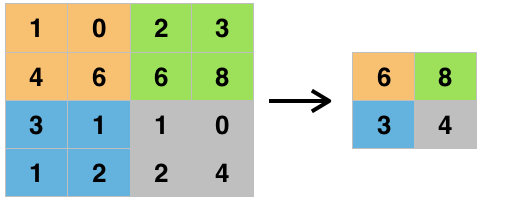
\includegraphics[width=0.6\linewidth]{Images/maxpool.png}
    \caption{Max pooling met 2x2 filter en stapgrootte 2}
    \label{fig:maxpool}
\end{figure}

Na \'e\'en of meerdere opeenvolgingen van filters, niet-lineaire en pooling lagen volgt in een traditionele convolutionele architectuur de laatste fase. Deze bestaat uit een aantal volledig verbonden lagen, gevolgd door een classificatielaag.

Trainen van dit netwerk kan gesuperviseerd met behulp van terugpropagatie, maar kan ook ongesuperviseerd. Deze laatste methode werkt veel sneller en heeft geen nood aan zeer grote gelabelde datasets. 
In vergelijking met gewone feedforward netwerken zijn CNN's in staat om veel sneller visuele concepten te leren, terwijl ze theoretisch slechts iets minder goede resultaten kunnen bekomen.
Bovendien is een CNN translatie-invariant omdat het op elk niveau gebruik maakt van rechthoekige regio's uit de vorige laag van het netwerk. Er is overlap tussen de verschillende regio's, wat leidt tot deze zeer interessante eigenschap.

\subsubsection[]{Concrete implementaties}
E\'en van de meest succesvolle toepassingen van CNN's is objectdetectie. Deze vooruitgang was vooral te wijten aan een onderzoek van Krizhevsky et al.\cite{Krizhevsky2012a} dat CNN's gebruikt voor het oplossen van de ImageNet challenge\cite{Russakovsky2014}.
Dit is een competitie over het classificeren van afbeeldingen in een aantal voorgedefini\"eerde categorie\"en. 

De gebruikte architectuur bestaat uit acht lagen waarvan vijf convolutioneel en drie volledig verbonden. Krizhevsky et al. gebruiken bovendien verschillende technieken om overfitten te vermijden. Als classificatielaag gebruiken ze softmax zodat het netwerk een kansverdeling over de verschillende categori\"een leert. Figuur \ref{fig:AlexNet} toont de architectuur en  is een variant op de standaardarchitectuur zoals hierboven beschreven. Dit netwerk was het best presterende netwerk voor de wedstrijd in 2012. Ondertussen zijn nog diepere architecturen voorgesteld die zowel op de ImageNet challenge als op recentere wedstrijden nog betere resultaten bekomen.

\begin{figure}[tb]
	\centering
	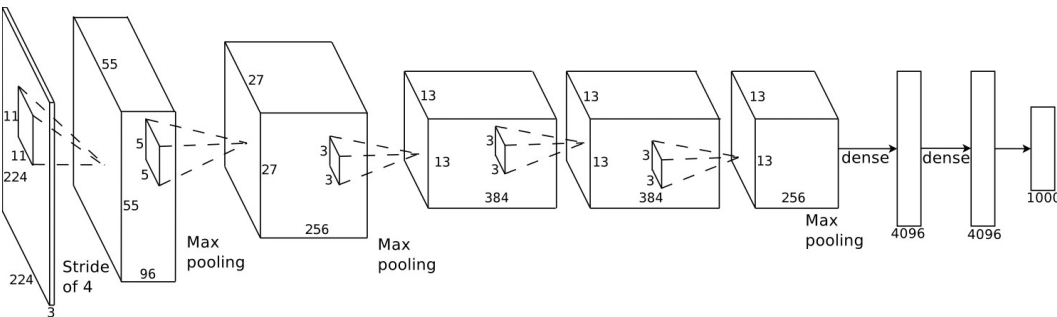
\includegraphics[width=\linewidth]{Images/cnn.PNG}
	\caption{Convolutioneel Neuraal Netwerk gebruikt voor classificatie van afbeeldingen\cite{Krizhevsky2012a}}
	\label{fig:AlexNet}
\end{figure}

Het recentere netwerk (VGGNet\cite{Arge2015}) bestaat uit meer lagen en is te gebruiken met behulp van publieke implementaties nin Caffe\cite{Jia2014}.
Figuur \ref{fig:alexvgg} toont een vergelijking tussen AlexNet en een versie van VGGNet met 13 gewichtslagen. De feature maps van verschillende outputlagen van dit netwerk dienen ook als input voor andere taken dan de ImageNet Challenge. Zo kan de output van de voorlaatste laag voor de softmaxlaag worden beschouwd als een representatievector voor de hele afbeelding. De outputs van de andere lagen stellen een aantal afbeeldingskenmerken voor op een niveau lager dan de volledige afbeelding.

\begin{figure}[tb]
	\centering
	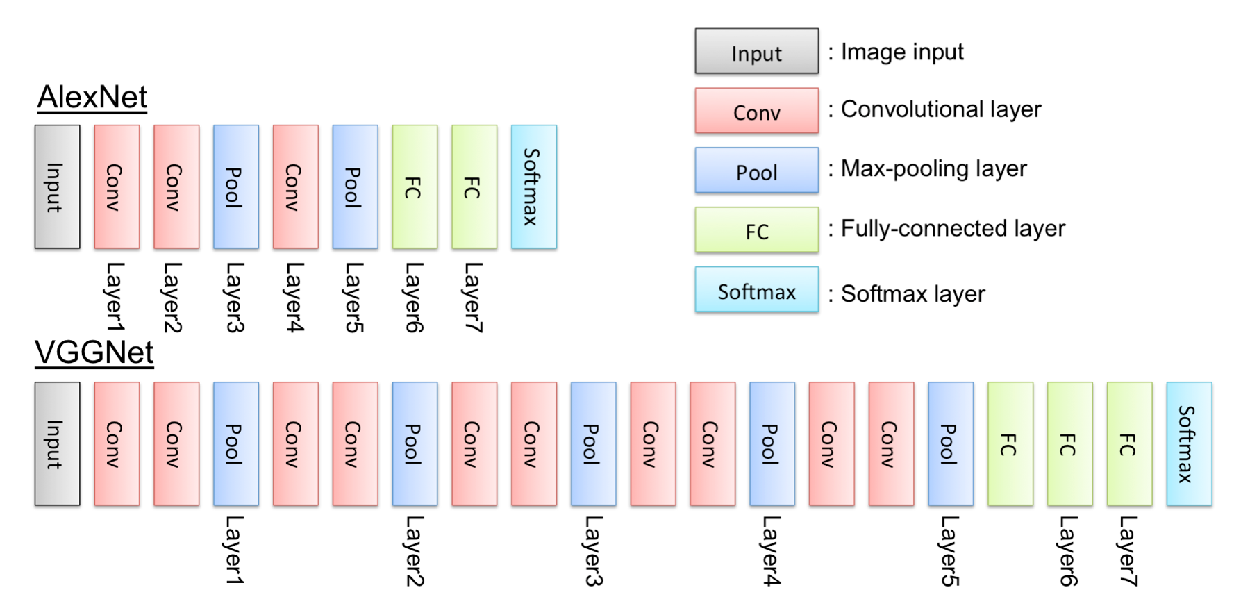
\includegraphics[width=\linewidth]{Images/alex_vgg.eps}
	\caption{Vergelijking van de architectuur van AlexNet en VGGNet}
	\label{fig:alexvgg}
\end{figure}

% RNN
\subsection{Recurrente Neurale Netwerken}
\subsubsection{Concept}
Recurrente neurale netwerken vormen een uitbreiding op standaard feedforward neurale netwerken. Ze kunnen, net zoals feedforward netwerken, getraind worden met terugpropagatie. Het grote verschil met feedforward netwerken is de terugkoppeling van uitvoer van de vorige invoer naar de verborgen lagen. Op figuur \ref{fig:rnn} is een ontrolling van een RNN over verschillende tijdstippen te zien. $U,V$ en $W$ stellen gewichtsmatrices voor. Het ontrollen van het netwerk komt neer op het uitschrijven van het netwerk over verschillende tijdstippen. De pijlen van links naar rechts op de afbeelding komen overeen met de terugkoppeling van de output uit de vorige stap.

De terugkoppeling zorgt ervoor dat het netwerk in staat is om informatie te onthouden, waardoor het mogelijk is om tijdsgerelateerde informatie te coderen. Daarom zijn ze geschikt om sequenti\"ele data, zoals tekst, te modelleren en te voorspellen. Recurrente neurale netwerken kunnen bijgevolg dienen als taalmodel\cite{Mikolov2010}.

\begin{figure}[tb]
    \centering
    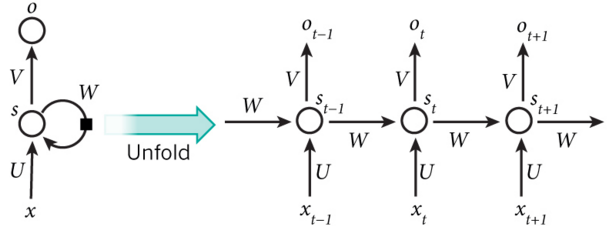
\includegraphics[width=\linewidth]{Images/rnn.PNG}
    \caption{Ontrolling van een recurrent neuraal netwerk\cite{RNNTutorial}}
    \label{fig:rnn}
\end{figure}

Het voorspellen van een zin met een RNN gebeurt woord per woord. Op basis van de eerder waargenomen woorden kan een softmaxlaag een kansverdeling berekenen voor het volgende woord. Met behulp van beam-search of het samplen van deze kansverdeling, is het netwerk in staat om zinnen te genereren. Het beam-search algoritme is een zoekalgoritme dat tijdens het zoeken net zoals breadth-first per niveau elke knoop gaat uitklappen. Het verschil met breadth-first is dat het enkel de hoogst-scorende expansies bijhoudt. Dit algoritme vindt niet altijd het optimale resultaat, maar zorgt wel voor een beperkt geheugengebruik.

Tijdens de trainingsfase bestaat de input van het netwerk uit woorden, voorgesteld als een vector. Deze vectoren kunnen gebaseerd zijn op one-hot codering, ze kunnen willekeurig zijn, of het kunnen vooraf getrainde word embeddings zijn zoals bijvoorbeeld \texttt{word2vec}\cite{Mikolov2013}. Deze codering van woorden tot vectoren zelf kan ook deel uitmaken van het netwerk. Als dit het geval is, kan de codering verbeteren tijdens de training met behulp van terugpropagatie.

\subsubsection{Problemen en oplossingen met RNN}

Een frequent probleem bij het trainen van recurrente netwerken is de complexiteit van het netwerk. Hoe complexer het netwerk, hoe groter de kans op ``overfitting''. Hierbij is het uiteindelijke netwerk te hard afgestemd op de trainingsdata, waardoor de precisie op de testdata achteruit gaat. Om dit probleem aan te pakken biedt Srivastava\cite{Srivastava2013} een oplossing. Hij introduceert ``dropout'' om dit fenomeen tegen te gaan. Bij het gebruik van dropout laat het netwerk tijdens het trainen een aantal neuronen vallen. Bij elk trainingsvoorbeeld zijn er een aantal gewichten die waarde 0 krijgen, waardoor ze niet bijdragen aan de training. Een willekeurig proces bepaalt welke neuronen nul zijn in elke stap. Dit proces is aangestuurd door een parameter die de kans op dropout aangeeft per neuron. Deze  kans kan verschillend zijn voor elke laag. Typisch is deze kans kleiner voor inputwaarden dan voor verborgen waarden.

Een tweede probleem is het gebrek aan aanpassing van de leersnelheid voor verschillende parameters. Hiervoor zijn een aantal oplossingen te vinden in de literatuur. Een eerste is het gebruik van ``Adagrad''\cite{Duchi2011}. Hierbij maakt het algoritme gebruik van formule \eqref{formule:adagrad} om de gewichten aan te passen. Hierdoor zullen parameters waarbij de gradi\"ent zeer groot is een lagere effectieve leersnelheid hebben dan parameters met een kleinere gradi\"ent. In de formule staat $w_t$ voor de gewichtsvector op tijdstip $t$, $dw$ is de gradi\"entvector, $\sigma$ is de leersnelheid, en $\epsilon$ is een afvlakkingsparameter die deling door nul voorkomt. Een probleem dat kan voorkomen bij het gebruik van ``Adagrad'' is dat het leerproces te vroeg stopt, omdat de aanpassingen aan de leersnelheid te agressief zijn.
 
\begin{equation}
    w_t = w_{t-1} - \sigma \frac{dw}{\sqrt{dw^2} + \epsilon}
    \label{formule:adagrad}
\end{equation}

Soms biedt deze methode onvoldoende verbetering, bijvoorbeeld wanneer er negen voorbeelden zijn met gradi\"ent $0.1$ voor een bepaalde parameter, en het tiende voorbeeld heeft waarde $-0.9$. Dan kan ``rmsprop''\cite{RMSprop} een oplossing bieden. Deze techniek maakt gebruik van een bewegend gemiddelde over alle voorbije gradi\"enten om ervoor te zorgen dat grote schommelingen in de gradi\"ent slechts een kleine verandering in de gewichten aanbrengen. Formules \eqref{rmsprop:start}-\eqref{formule:rmsprop} toont hoe dit exact in zijn werk gaat. $\rho$ is de afvlakkingsparameter voor het bewegend gemiddelde, $\sigma$ is de leersnelheid, $a_t$ is de gemiddelde gradi\"ent op tijdstip $t$, $dw$ is de gradi\"ent en $w$ is de gewichtsvector. Ook hier vermijdt $\epsilon$ een mogelijke deling door nul.

\begin{eqnarray}
\vspace{-3mm}
    \label{rmsprop:start}
    a_t & = & \rho  a_{t-1} + (1 - \rho)dw^2 \\
    w_t & = &  - \sigma \frac{dw}{\sqrt{a_t} + \epsilon}
    \label{formule:rmsprop}
    \vspace{-3mm}
\end{eqnarray}

Een ander probleem met ``Adagrad'' is dat de effectieve leersnelheid naar nul convergeert naarmate de training langer duurt. ``Adadelta''\cite{Zeiler2012} biedt hiervoor een oplossing door, net als ``rmsprop'' gebruik te maken van een bewegend gemiddelde, zowel voor gradi\"ent als voor de gewichten. Door het gebruik van dit tweede gemiddelde is het niet nodig om expliciet een leersnelheid te defini\"eren. Formules \eqref{adadelta:start}-\eqref{formule:adadelta} tonen de exacte berekening van gewichtsupdates bij het gebruik van adadelta. $a_t$, $\rho$, $\epsilon$, $w$ en $dw$ zijn hetzelfde gedefini\"eerd als bij adagrad. $a_{w,t}$ is het bewegende gemiddelde van de gewichtsupdates op tijdstip $t$ en $\Delta w_t$ is de aanpassing die gebeurt aan de gewichten op tijdstip $t$.

\begin{eqnarray}
\vspace{-3mm}
    \label{adadelta:start}
    a_t & = & \rho  a_{t-1} + (1 - \rho)dw^2 \\
    \Delta w_t & = & - \frac{\sqrt{a_{w,(t-1)} + \epsilon}}{\sqrt{a_{t-1}}}dw \\
    a_{wt} & = & \rho  a_{w,(t-1)} + (1 - \rho)\Delta w_t^2 \\
    w_t & = & w_{t-1} + \Delta w_t
    \label{formule:adadelta}
    \vspace{-3mm}
\end{eqnarray}


Twee andere vaak voorkomende problemen bij het trainen van recurrente neurale netwerken zijn exploderende en uitdovende gradi\"enten, waarbij de gradi\"ent van de fout tijdens de training enorm toeneemt, respectievelijk afneemt. Hiervoor zijn een aantal mogelijke oplossingen.

``Gradient clipping'' vormt een eerste oplossing zoals voorgesteld door Pascanu et al.\cite{Pascanu2012}. Deze methode verkort de gradi\"entvector zodra de lengte van die vector boven een bepaalde drempel $t$ ligt en lost zo het probleem van exploderende gradi\"enten op. De gewichtsupdate vindt dan plaats in de dezelfde richting, maar de norm is aangepast naar de maximale waarde $t$. Voor een vector $\mathbf{g}$ komt dit neer op volgende resulterende gradi\"entvector $\mathbf{\hat{g}}$:

\begin{equation}
    \mathbf{\hat{g}} = \frac{t}{||\mathbf{g}||}\mathbf{g}
\end{equation}

Het gebruik van Rectified Linear Units of ReLu-encodering biedt een oplossing voor het probleem van uitdovende gradi\"enten. Dit is een activatiefunctie die werkt volgens formule $ReLu(x) = max(x,0)$. Deze functie is zeer eenvoudig te berekenen en vermijdt uitdovende grade\"enten, in tegenstelling tot niet-lineaire functies zoals een sigmo\"ide of een hyperbolische tangens\cite{Glorot2011}.

Door deze problemen is het voor een RNN moeilijk om informatie te onthouden op langere termijn. Hochreiter et al.\cite{SeppHochreiter1997} bieden met Long Short Term Memory netwerken een andere mogelijke oplossing voor dit probleem.

% LSTM
\subsection{Long Short Term Memory Neurale Netwerken}
\label{sub:lstm}
Long Short Term Memory (LSTM) is een vorm van RNN die geheugencellen bevat. Door deze cellen is het netwerk in staat om op lange termijn informatie over de input bij te houden. Elk LSTM-geheugencel heeft een aantal poorten of gates om te bepalen of de input moet onthouden worden, en of een vorige waarde moet bijgehouden of vergeten worden. De output van de cellen is bijgevolg afhankelijk van alle eerder geobserveerde inputs. Figuur \ref{fig:lstm} toont hoe een LSTM-blok er uitziet.\cite{SeppHochreiter1997,Google}

Op de figuur is duidelijk te zien hoe zowel input als output zijn teruggekoppeld naar de verschillende poorten. De waarde van die poorten hangt dus af van de vorige voorspellingen van de nieuwe input.

Formules \eqref{lstm-memory-start}-\eqref{lstm-memory} geven de exacte berekeningen weer die elke stap gebeuren. In deze formules zijn alle $W_{ij}$ gewichtsmatrices, $\sigma$ en $h$ zijn transferfuncties. $x$ is de input van het netwerk, $m_t$ is de output op tijdstip $t$ en $i'_t$, $f'_t$ en $o'_t$ zijn de waarden van respectievelijk input-, vergeet- en outputpoort op tijdstip $t$. $c'_t$ is de waarde van de geheugencel op tijdstip $t$ en $p_t$ is de uiteindelijke voorspelling van het netwerk op tijdstip $t$. De $\odot$ operator stelt een puntsgewijze vermenigvuldiging tussen twee vectoren voor.


\begin{figure}[tb]
    \centering
    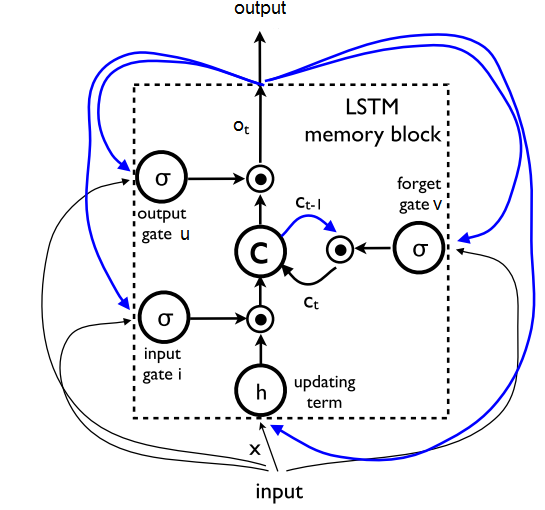
\includegraphics[width=\linewidth]{Images/lstm.PNG}
    \caption{Long Short Term Memory geheugencel}
    \label{fig:lstm}
\end{figure}

\begin{eqnarray}
\vspace{-3mm}
\label{lstm-memory-start}
i_t' & = & \sigma (W_{ix} x_t + W_{im} m_{t-1}) \label{lstm-input} \\
f_t' & = & \sigma (W_{fx} x_t + W_{fm} m_{t-1}) \\
o_t' & = & \sigma (W_{ox} x_t + W_{om} m_{t-1}) \\
c_t' & = & f_t' \odot c_{t-1}' + i_t' \odot h(W_{cx} x_t + \nonumber \\
&   & + W_{cm} m_{t-1}) \\
m_t & = & o_t' \odot c_t'\\
\label{lstm-memory}
\vspace{-3mm}
\end{eqnarray}

LSTM-netwerken worden net als RNN gebruikt als taalmodellen en zorgen over het algemeen voor hogere kwaliteit. Dit komt doordat een LSTM-netwerk over een langere periode dan een eenvoudig RNN informatie kan onthouden. Dit maakt het modelleren van sequenties met events, die gescheiden zijn door een langere periode, mogelijk.


\section{Statistische concepten}

% LDA
\subsection{Latent Dirichlet Allocation}
Latent Dirichlet Allocation\cite{Blei2012} is een generatief probabilistisch model voor discrete data. E\'en van de meest gebruikte toepassingen hiervan is het modelleren van een een verdeling van onderwerpen in een set van tekstdocumenten. De onderliggende veronderstelling is dat elk document een zekere kansverdeling heeft over alle mogelijke onderwerpen. Deze onderwerpen hebben op hun beurt een kansverdeling over alle mogelijke woorden. Zo beschrijft formule \ref{formule:lda} de kans dat een bepaald document $d_j$ een bepaald woord $w_i$ bevat. $z_k$ is hier het $k^{de}$ onderwerp. Voor documenten die bijvoorbeeld sportevenementen beschrijven, zullen woorden als \texttt{wedstrijd, score, bal, spannend} een hogere score krijgen.

\begin{equation}
    P(w_i | d_j) = \sum\limits_{k=0}^{n_{topics}}P(w_i|z_k)P(z_k|d_j)
    \label{formule:lda}
\end{equation}

Het generatieve aspect van LDA is te zien in algoritme \ref{algo:lda} en is ook ge\"illustreerd in figuur \ref{fig:lda}. Op basis van twee Dirichlet priors $\alpha$ en $\beta$ samplet het algoritme een kansverdeling over de onderwerpen per document ($\theta$) en een kansverdeling over de woorden voor elk onderwerp ($\phi$). Deze priors geven de onzekerheid over de variabelen ($\theta$ en $\phi$) weer en dienen als basis voor een Dirichletverdeling\cite{Huang}. Een mogelijke interpretatie $\alpha$ is het aantal observaties van de verschillende topics alvorens het document in kwestie is gezien. Hetzelfde met $\beta$, dat het voorafgaand aantal samples van een bepaald woord uit een bepaald topic voorstelt. Het algoritme samplet voor elke positie $i$ in een document $j$ een onderwerp ($z_{ji}$) uit $\theta$. Het samplen van de woordverdeling voor dit onderwerp leidt tot het woord $w_{ji}$\cite{LDAsien}.

\begin{algorithm}
\caption{Generatief aspect van LDA}
\begin{algorithmic} 
\STATE sample $K$ keer  $\phi \sim Dirichlet(\beta)$
\FORALL{document $d_j$}
\STATE sample $\theta \sim Dirichlet(\alpha)$
\FORALL{woord $i \in d_j$}
\STATE sample $z_{ji} \sim Multinomial(\theta)$
\STATE sample $w_{ji} \sim Multinomial(\phi,z_{ji})$
\ENDFOR
\ENDFOR
\end{algorithmic}
\label{algo:lda}
\end{algorithm}

\begin{figure}[tb]
    \centering
    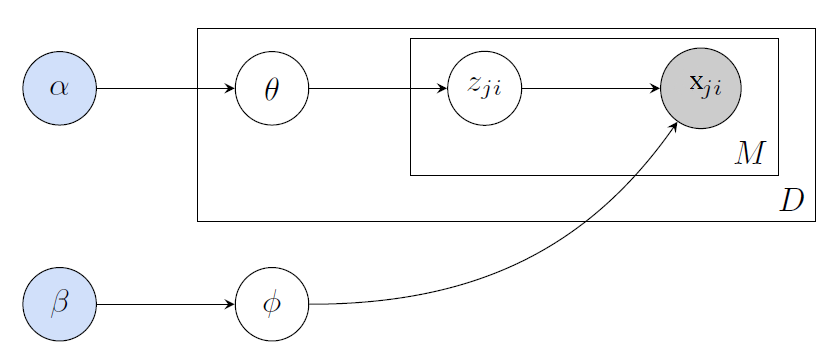
\includegraphics[width=\linewidth]{Images/lda.png}
    \caption{Grafische weergave van LDA}
    \label{fig:lda}
\end{figure}

Trainen van een LDA-model gebeurt met een Markov chain Monte Carlo algoritme. Dit type algoritme construeert een Markovketen met als doel een kansdichtheidsfunctie te benaderen. In een Markovketen is de volgende stap enkel afhankelijk van de huidige toestand, waardoor het berekenen minder complex is. De meest gebruikte techniek om een LDA-model te benaderen is Gibbs sampling. Het uiteindelijke doel is het benaderen van de kansverdelingen $\theta$ en $\phi$.

Het trainen met Gibbs sampling begint met een random initialisatie van de onderwerpverdeling voor elk document. Daarna itereert het algoritme over elk woord in elk document. Het berekent de kansverdeling over de verschillende topics, gebaseerd op de onderwerpen van de andere woorden in de collectie (update stap). Formule \eqref{lda:update} toont de exacte berekening. Hierbij is $n_{j,k}$ het aantal toekenningen van onderwerp $k$ aan een woord in document $d_j$. $n_{j,k,\neg i}$ is het aantal keer dat topic $k$ is toegekend aan een woord in document $d_j$, woord $w_{ji}$ niet meegeteld. $n_{j,\cdot,\neg i}$ is de som van $n_{j,k,\neg i}$ over alle $K$ topics. $v_{k,w_{ji}}$ is het aantal associaties van woord $w_{ji}$ met topic $k$ in alle documenten. $v_{k,w_{ji}}$ is hetzelfde getal, maar dan zonder het huidige woord $w_ji$ mee te tellen. $v_{k,\cdot,\neg}$ is het totaal aantal woorden die bij topic $k$ horen, zonder $w_{ji}$ mee te tellen.

\begin{equation}
    P(z_{ji} = k | \mathbf{z}_{\neg ji}, \mathbf{w}, \alpha, \beta) \propto \frac{n_{j,k,\neg i} + \alpha}{n_{j, \cdot, \neg i} + K \alpha} \cdot \frac{v_{k,w_{ji}, \neg}+ \beta}{v_{k,\cdot,\neg} + |V|\beta}
    \label{lda:update}
\end{equation}

Op basis van deze kansverdeling samplet formule \eqref{lda:sample} een nieuw topic gesampled voor het huidige woord. Dit proces van updaten en samplen herhaalt zich tot er convergentie plaatsvindt. De geleerde onderwerpverdelingen voor elk woord dienen dan als basis voor de onderwerpverdelingen voor elk document en de woordverdelingen per topic. Formule \eqref{form:doctopic} toont de berekening van de document-onderwerpverdeling. Formule \eqref{form:topicword} bevat deze voor topic-woordverdelingen. De symbolen hebben dezelfde betekenis als eerder beschreven.

\begin{equation}
    z_{ji} \sim  P(z_{ji} = k | \mathbf{z}_{\neg ji}, \mathbf{w}, \alpha, \beta)
    \label{lda:sample}
\end{equation}

\begin{equation}
    P(z_k|d_j) = \theta_{j,k} = \frac{n_{j,k} + \alpha}{\sum_{k^*=1}^K n_j,k^* + K\alpha}
    \label{form:doctopic}
\end{equation}

\begin{equation}
    P(w_i|z_k) = \phi_{k,i} = \frac{v_{k,w_i} + \beta}{\sum_{i^*=1}^{|V|} v_k,w_{i^*} + |V|\beta}
    \label{form:topicword}
\end{equation}

Het meest interessante voor deze masterproef zijn de onderwerpverdelingen per document. Deze kunnen dienen als extra semantische informatie. De systemen kunnen op basis van onderverdelingen een verband leren tussen de onderwerpen die voorkomen in de beschrijvingen en de concepten die aanwezig zijn in de afbeelding. 


%  Stacked CCA
\subsection{Canonical Correlation Analysis}
\label{sub:stackedcca}
Canonical Correlation Analysis (CCA) is een methode die basisvectoren probeert te vinden voor twee gerelateerde datasets. De bedoeling is om, bij projectie van overeenkomstige elementen uit beide datasets, een maximale lineaire correlatie te bekomen tussen de twee projecties. 
Op basis van singulierewaardenontbinding (SWO) van de twee datasets is het mogelijk om deze ruimte te benaderen. Door het gebruik van singuliere waarden is het mogelijk om projecties in de tussenliggende ruimte te reduceren tot hun $n$ eerste componenten. Dit komt doordat een SWO de dimensies rangschikt van dominant naar minder dominant. Weenink\cite{Weenink2003} beschrijft de theoretische uitwerking en oplossingsmethodes.

In het onderzoek naar afbeeldingsbeschrijving kan dit bijvoorbeeld leiden tot een multimodale projectie van afbeeldings- en beschrijvingsrepresentatie.

\paragraph{Stacked CCA}

Stacked Auxiliary Embedding\cite{Gong2014} kan op basis van extra informatie een verbeterde projectie maken ten opzichte van gewone CCA. Een voorbeeld hiervan is een dataset van geannoteerde foto's, versterkt met per foto een set van stukjes van de foto met een bijbehorende beschrijving. De representaties van de foto's en annotaties uit de dataset kunnen verbeteren door gebruik te maken van de informatie uit de extra dataset.

Om de uiteindelijke augmentatie te bereiken, zijn er een aantal stappen nodig. Uit de extra dataset volgt een eerste set van CCA-projecties ($A$, $B$). Daarna volgt een projectie van de originele dataset ($X$, $Y$) naar de multimodale ruimte, door vermenigvuldiging met $A$ en $B$. Dit resulteert in projecties $AX$ en $BY$. Vervolgens transformeert een lineaire functie $\phi(x)$ de waarden $AX$ en $BY$ zoals de originele paper voorstelt.

Aaneensluiting van de originele dataset met het resultaat van de niet-lineaire transformatie leidt tot $\hat{X} = [X, \phi(XA)], \hat{Y} = [Y, \phi(YB)]$. Een laatste stap in het proces berekent een CCA-projectie die gebaseerd is op $\hat{X}$ en $\hat{Y}$, wat resulteert in $U$ en $V$.

Om de dimensionaliteit van de projectie te verhogen gebruikt de paper voor $\phi(x)$ een random Fourier Feature (RFF). Deze RFF is een functie die de gemiddelde afstand tot de vijftigste dichtste buur van de inputvector gebruikt. Voor elke foto en beschrijving kijkt het algoritme welke andere foto of beschrijving de vijftigste dichtste buur is, om vervolgens het gemiddelde te nemen van alle afstanden. De exacte berekening is $\phi(\mathbf{x})=\sqrt{2}cos(\mathbf{x}R+\mathbf{b})$. Hierin is $R$ een matrix die verkregen door sampling van een normaalverdeling met gemiddelde 0, en standaardafwijking $\sigma^2$, waarbij $\sigma$ overeen komt met de eerder berekende gemiddelde afstand. Vector $b$ is resultaat van sampling uit een uniforme verdeling [0,1].

De projectie van een ongeziene afbeelding is het resultaat van het achtereenvolgens uitvoeren van alle transformaties. Voor vector $\mathbf{x}$ geeft dit $\mathbf{\hat{x}} = U[\mathbf{x}, \phi(A\mathbf{x})]$. Deze representatie vormt dan een verbeterde versie van de originele afbeeldingsrepresentatie, wat nuttig is voor bijvoorbeeld het opzoeken van afbeeldingen.
